\chapter{HASIL DAN PEMBAHASAN}

\vspace{1cm}
\section{Area Studi}
\hspace{1,2cm}
Terdapat dua area studi yang dilakukan pada penelitian ini, yaitu Kebun Pendidikan dan Penelitian Kelapa Sawit milik Institut Pertanian Bogor-Cargil yang berlokasi di Jonggol, Jawa Barat dan Universitas Gunadarma di Penajam Paser Utara, Kalimantan Timur yang memiliki lahan yang ditanami pohon kelapa sawit.

Area studi ini secara umum mencakup untuk pengambilan data citra pohon kelapa sawit sebagai dataset primer. Tabel \ref{tbl:Data-Lokasi-dan-Luasan-Area-Studi} menampilkan lokasi koordinat dan luasan lahan yang diambil sebagai citra pohon kelapa sawit.

%%%%%%%%%%%%%%%%%%%%%%%TABEL SEDERHANA%%%%%%%%%%%%%%%%%%%%%%%%%
\begin{singlespace}
	\begin{table}[H]
		\centering
		\caption{Data Lokasi dan Luasan Area Studi}
		\label{tbl:Data-Lokasi-dan-Luasan-Area-Studi}
		\begin{tabular}{|p{4cm}|p{4cm}|p{4cm}|}
			\hline
			\rowcolor[HTML]{D9D9D9}
			Area Studi                                                                         & Lokasi Koordinat (Latitude, Longitude) & Luasan Lahan (ha) \\ \hline

			Kebun Pendidikan dan Penelitian Kelapa Sawit milik Institut Pertanian Bogor-Cargil & -6.4277942, 106.8418378                                                          & 63,48                                                          \\ \hline
			
			Universitas Gunadarma di Penajam Paser Utara, Kalimantan Timur                     & -1.318495, 116.6678405                                                           & $\approx$ 18                                                           \\ \hline
			\end{tabular}
	\end{table}
\end{singlespace}
%%%%%%%%%%%%%%%%%%%%%%%TABEL SEDERHANA%%%%%%%%%%%%%%%%%%%%%%%%%

Pengambilan citra pada area studi diambil dengan menggunakan DJI Mavic 2 Pro dari ketinggian 100 m di atas permukaan tanah dengan pakar atau pilot drone yang sudah tersertifikasi. Pada tahap pengujian pada sistem untuk mendeteksi dan menghitung, serta titik koordinat latitude-longitude dari setiap pohon kelapa sawit menggunakan area Kebun Pendidikan dan Penelitian Kelapa Sawit milik Institut Pertanian Bogor-Cargil Blok 1, 2, 3, dan 4. Pada proses pengambilan citra untuk dataset primer pada area studi lahan pada Kebun Pendidikan dan Penelitian Kelapa Sawit milik Institut Pertanian Bogor-Cargil berhasil ditangkap area blok 3 dan 4 dari total 4 blok. Peta sebaran area inisialisasi lahan pada kebun ini seperti pada Gambar \ref{img:Peta-Sebaran-Area-Inisialisasi-Lahan-Kebun} yang memiliki 5670 pohon tanam kelapa sawit berdasarkan hasil wawancara di lapangan pada area studi Kebun Pendidikan dan Penelitian Kelapa Sawit milik Institut Pertanian Bogor-Cargil.

%%%%%%%%%%%%%%%%%%%%%%%%%% GAMBAR %%%%%%%%%%%%%%%%%%%%%%%%%%%%%%
\begin{figure}[H]
	\vspace{-0.1cm}
	%\rule{\columnwidth}{0.1pt}
	\begin{center}
		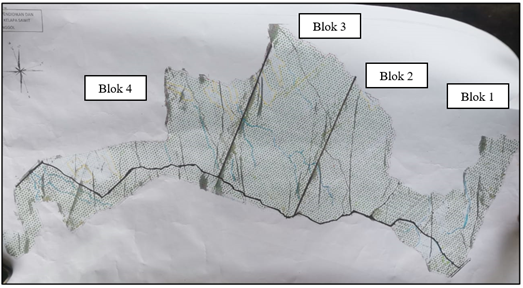
\includegraphics[width=1\columnwidth]{bab4/Gambar/Picture1.png}
	\end{center}
	\vspace{-0.2cm}
	%\rule{\columnwidth}{0.1pt}
	\captionsetup{justification=centering}
	\caption{Peta Sebaran Area Inisialisasi Lahan Kebun Pendidikan dan Penelitian Kelapa Sawit milik Institut Pertanian Bogor-Cargil}\label{img:Peta-Sebaran-Area-Inisialisasi-Lahan-Kebun}
\end{figure}
%%%%%%%%%%%%%%%%%%%%%%%%%% GAMBAR %%%%%%%%%%%%%%%%%%%%%%%%%%%%%%

Area lahan yang berhasil ditangkap pada kebun ini berada pada area studi blok 3 dan blok 4. Area studi yang digunakan untuk dataset primer yang digunakan blok 3 pada Gambar 3.6 dan blok 4 pada Gambar 3.7. dengan total luas sebesar 37,51 hektar, dan pengujian digunakan blok 1 (Gambar 4.2), 2 (Gambar 4.3), 3, dan 4 seperti pada Tabel \ref{tbl:Area-Studi-Yang-Berhasil-Ditangkap-Menjadi-CItra-Area-Pohon-Kelapa-Sawit-Dengan-Drone} dengan total luas area 63,48 hektar pada Kebun Pendidikan dan Penelitian Kelapa Sawit Institut Pertanian Bogor-Cargil dengan perhitungan luas area menggunakan bantuan layanan DroneDeploy.

%%%%%%%%%%%%%%%%%%%%%%%TABEL SEDERHANA%%%%%%%%%%%%%%%%%%%%%%%%%
\begin{singlespace}
	\begin{table}[H]
		\centering
		\caption{Area Studi yang Berhasil Ditangkap menjadi Citra Area Pohon Kelapa Sawit dengan Drone}
		\label{tbl:Area-Studi-Yang-Berhasil-Ditangkap-Menjadi-CItra-Area-Pohon-Kelapa-Sawit-Dengan-Drone}
		\begin{tabular}{|ll|l|}
			\hline
			\rowcolor[HTML]{D9D9D9} 
			\multicolumn{1}{|l|}{\cellcolor[HTML]{D9D9D9}No.} & Area   & Luas Area (ha) \\ \hline
			\multicolumn{1}{|l|}{1}                           & Blok 1 & 14,66          \\ \hline
			\multicolumn{1}{|l|}{2}                           & Blok 2 & 11,31          \\ \hline
			\multicolumn{1}{|l|}{3}                           & Blok 3 & 18,20          \\ \hline
			\multicolumn{1}{|l|}{4}                           & Blok 4 & 19,31          \\ \hline
			\multicolumn{2}{|l|}{Total}                                & 63,48          \\ \hline
		\end{tabular}
	\end{table}
\end{singlespace}
%%%%%%%%%%%%%%%%%%%%%%%TABEL SEDERHANA%%%%%%%%%%%%%%%%%%%%%%%%%

%%%%%%%%%%%%%%%%%%%%%%%%%% GAMBAR %%%%%%%%%%%%%%%%%%%%%%%%%%%%%%
\begin{figure}[H]
	\vspace{-0.1cm}
	%\rule{\columnwidth}{0.1pt}
	\begin{center}
		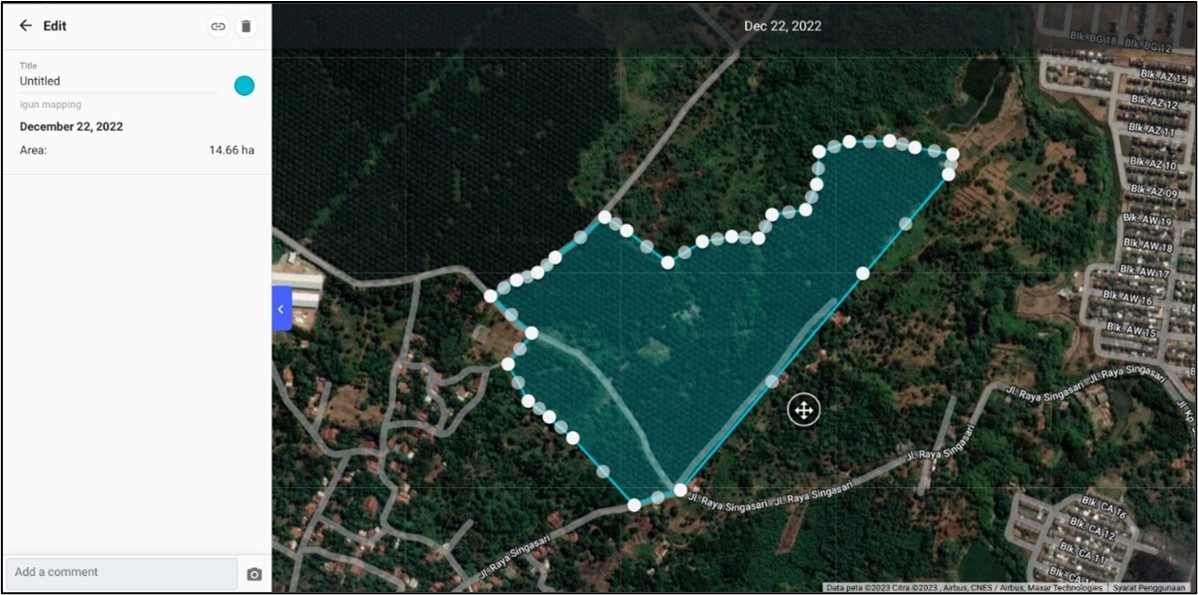
\includegraphics[width=0.7\columnwidth]{bab4/Gambar/Picture2.jpg}
	\end{center}
	\vspace{-0.2cm}
	%\rule{\columnwidth}{0.1pt}
	\captionsetup{justification=centering}
	\caption{Luas Area Blok 1 Kebun Pendidikan dan Penelitian Kelapa Sawit Institut Pertanian Bogor-Cargil}\label{img:Luas-Area-Blok-1-Kebun-Pendidikan}
\end{figure}
%%%%%%%%%%%%%%%%%%%%%%%%%% GAMBAR %%%%%%%%%%%%%%%%%%%%%%%%%%%%%%

%%%%%%%%%%%%%%%%%%%%%%%%%% GAMBAR %%%%%%%%%%%%%%%%%%%%%%%%%%%%%%
\begin{figure}[H]
	\vspace{-0.1cm}
	%\rule{\columnwidth}{0.1pt}
	\begin{center}
		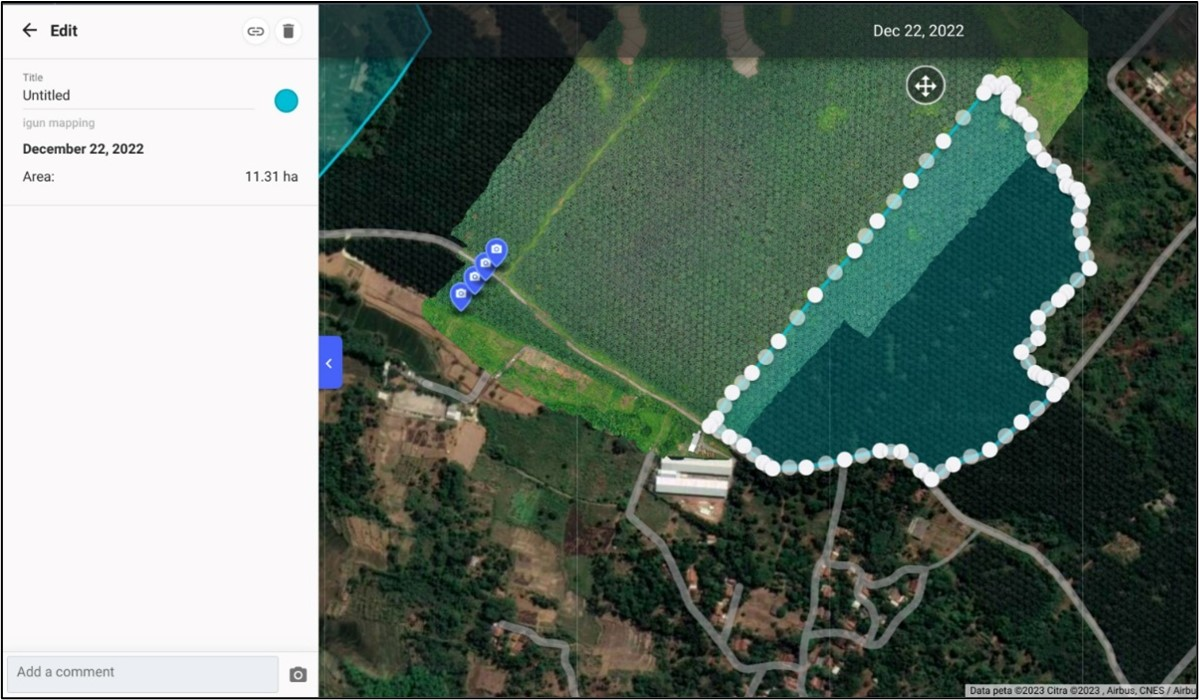
\includegraphics[width=0.7\columnwidth]{bab4/Gambar/Picture3.jpg}
	\end{center}
	\vspace{-0.2cm}
	%\rule{\columnwidth}{0.1pt}
	\captionsetup{justification=centering}
	\caption{Luas Area Blok 2 Kebun Pendidikan dan Penelitian Kelapa Sawit Institut Pertanian Bogor-Cargil}\label{img:Luas-Area-Blok-2-Kebun-Pendidikan}
\end{figure}
%%%%%%%%%%%%%%%%%%%%%%%%%% GAMBAR %%%%%%%%%%%%%%%%%%%%%%%%%%%%%%

\section{Persiapan Data}
\hspace{1,2cm}
Persiapan data, yang dikenal dengan \textit{data preprocessing} adalah tahap yang penting untuk menyiapkan data untuk dapat digunakan dalam modeling dengan \textit{deep learning}. Persiapan data meliputi persiapan dataset primer dan sekunder untuk dapat digunakan.

\subsection{Deskripsi Dataset dan Pemilihan}
\hspace{1,2cm}
Akuisisi citra area pohon kelapa sawit menjadi penting karena berhubungan hasil memindai, menangkap (\textit{capture}), atau menjadi suatu foto citra yang dapat digunakan untuk dataset. Citra area pohon kelapa sawit pada penelitian ini dibagi menjadi dua, yaitu citra untuk dataset primer dan sekunder.

\subsubsection{Dataset Primer}
\hspace{1,2cm}
Dataset primer digunakan untuk membangun atau memberikan anotasi atau label oil palm pada citra gambar. Hasil gambar citra pohon kelapa sawit dari dua area studi memiliki format citra yang sama, yaitu *.jpg. Data citra dari Kebun Pendidikan dan Penelitian Kelapa Sawit milik Institut Pertanian Bogor-Cargil yang diambil dari blok 3 dan 4 terdiri dari 69 citra atau gambar, sedangkan jumlah citra yang dihasilkan dari area kelapa sawit berjumlah 205 citra dengan dimensi ukuran citra sebesar 5472 x 3078 px, seperti pada Tabel \ref{tbl:Jumlah-Citra-Dari-Dua-Area-Studi}

Total citra dataset primer dari dua area studi seperti pada Tabel \ref{tbl:Jumlah-Citra-Dari-Dua-Area-Studi} berikut.

%%%%%%%%%%%%%%%%%%%%%%%TABEL SEDERHANA%%%%%%%%%%%%%%%%%%%%%%%%%
\begin{singlespace}
	\begin{table}[H]
		\centering
		\caption{Jumlah Citra dari Dua Area Studi}
		\label{tbl:Jumlah-Citra-Dari-Dua-Area-Studi}
		\begin{tabular}{|p{4cm}|p{4cm}|p{4cm}|}
			\hline
			\rowcolor[HTML]{D9D9D9} 
			Area Studi                                                                         & Jumlah Citra & Luas Area (ha) \\ \hline
			Kebun Pendidikan dan Penelitian Kelapa Sawit milik Institut Pertanian Bogor-Cargil & 69           & 14,66          \\ \hline
			Universitas Gunadarma di Penajam Paser Utara, Kalimantan Timur                     & 205          & 11,31          \\ \hline
		\end{tabular}
	\end{table}
\end{singlespace}
%%%%%%%%%%%%%%%%%%%%%%%TABEL SEDERHANA%%%%%%%%%%%%%%%%%%%%%%%%%

Hasil citra dari area studi Universitas Gunadarma dengan jumlah 205 citra atau gambar ini digunakan untuk dataset primer dengan memberikan anotasi atau pemberian label secara otomatis yang dilakukan dalam penelitian ini.  Adapun citra sampel area studi dari Universitas Gunadarma tampak pada Gambar \ref{img:Hasil-Citra-Sampel-Universitas-Gunadarma-1} dan citra sampel Kebun Pendidikan dan Penelitian Kelapa Sawit milik Institut Pertanian Bogor-Cargil tampak pada Gambar \ref{img:Hasil-Citra-Sampel-Universitas-Gunadarma-2}

%%%%%%%%%%%%%%%%%%%%%%%%%% GAMBAR %%%%%%%%%%%%%%%%%%%%%%%%%%%%%%
\begin{figure}[H]
	\vspace{-0.1cm}
	%\rule{\columnwidth}{0.1pt}
	\begin{center}
		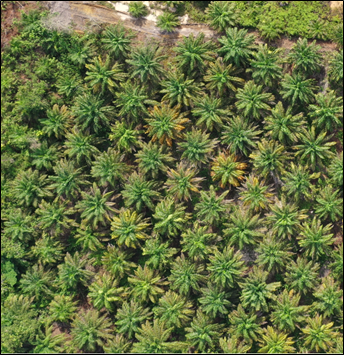
\includegraphics[width=0.6\columnwidth]{bab4/Gambar/Picture4.1.png}
		\hspace{1cm}
		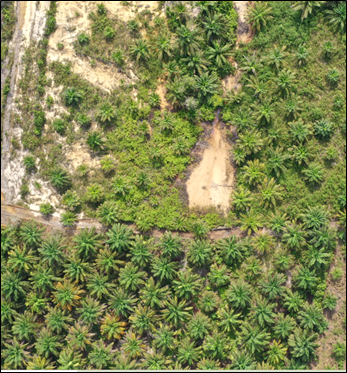
\includegraphics[width=0.6\columnwidth]{bab4/Gambar/Picture4.2.png}
	\end{center}
	\vspace{-0.2cm}
	%\rule{\columnwidth}{0.1pt}
	\captionsetup{justification=centering}
	\caption{Hasil Citra Sampel Universitas Gunadarma di Penajam Paser Utara, Kalimantan Timur}\label{img:Hasil-Citra-Sampel-Universitas-Gunadarma-1}
\end{figure}
%%%%%%%%%%%%%%%%%%%%%%%%%% GAMBAR %%%%%%%%%%%%%%%%%%%%%%%%%%%%%%

%%%%%%%%%%%%%%%%%%%%%%%%%% GAMBAR %%%%%%%%%%%%%%%%%%%%%%%%%%%%%%
\begin{figure}[H]
	\vspace{-0.1cm}
	%\rule{\columnwidth}{0.1pt}
	\begin{center}
		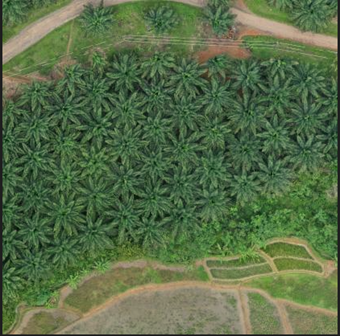
\includegraphics[width=0.6\columnwidth]{bab4/Gambar/Picture5.1.png}
		\hspace{1cm}
		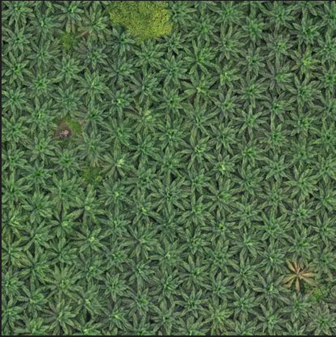
\includegraphics[width=0.6\columnwidth]{bab4/Gambar/Picture5.2.png}
	\end{center}
	\vspace{-0.2cm}
	%\rule{\columnwidth}{0.1pt}
	\captionsetup{justification=centering}
	\caption{Hasil Citra Sampel Universitas Gunadarma di Penajam Paser Utara, Kalimantan Timur}\label{img:Hasil-Citra-Sampel-Universitas-Gunadarma-2}
\end{figure}
%%%%%%%%%%%%%%%%%%%%%%%%%% GAMBAR %%%%%%%%%%%%%%%%%%%%%%%%%%%%%%

\subsubsection{Dataset Sekunder}
\hspace{1,2cm}
Data sekunder yang digunakan sudah memiliki label atau anotasi sebagai pohon kelapa sawit "oil palm". Data berjumlah 1795 citra yang sudah memiliki kotak batas atau \textit{bounding box} dengan kelas \textit{oil palm}. Data sekunder digunakan untuk menambah data pada sata proses pelatihan, validasi dan pengujian. Data tersebut semakin bervariasi, maka keterwakilan data pada citra yang berupa objek pohon kelapa sawit semakin baik. Dataset sekunder dapat diakses secara daring dan dapat digunakan secara \textit{free} atau \textit{open source} melalui sistem berbasis web bernama roboflow.

Data sample pada dataset sekunder yang sudah memiliki \textit{bounding box} yang diberi label oil palm, seperti pada Gambar 4.6.

